\section{Getting started with DySMo}\label{kap2}

DySMo supports different modeling tools and an arbitrary number of mode switches. This chapter gives you a design overview and shows you how your models have to be prepared to use them as variable-structure models in the given framework.

\subsection{DySMo's general design}

The basic idea of DySMo consists of creating variable-structure models by using integrated standard simulation tools and thus using already implemented models, too. Further the framework should always disclose what happens at any point during simulation. This section gives a brief introduction into the structural design of DySMo.\\
\\
A variable-structure model consists of different modes whereby every mode is a separately executable model. At any point during simulation one of the modes is active and determines the dynamic behavior of the whole variable-structure model (see Figure \ref{fig:simulation}). The mode switches can occur during simulation using transitions. Therefore, a control is needed which manages the mode switches, and this control is provided by the framework. The framework at the current state only allows modes in the highest level of hierarchy, modes consisting of further modes cannot be implemented (directly).

 \begin{figure}[htb]
 \centering
 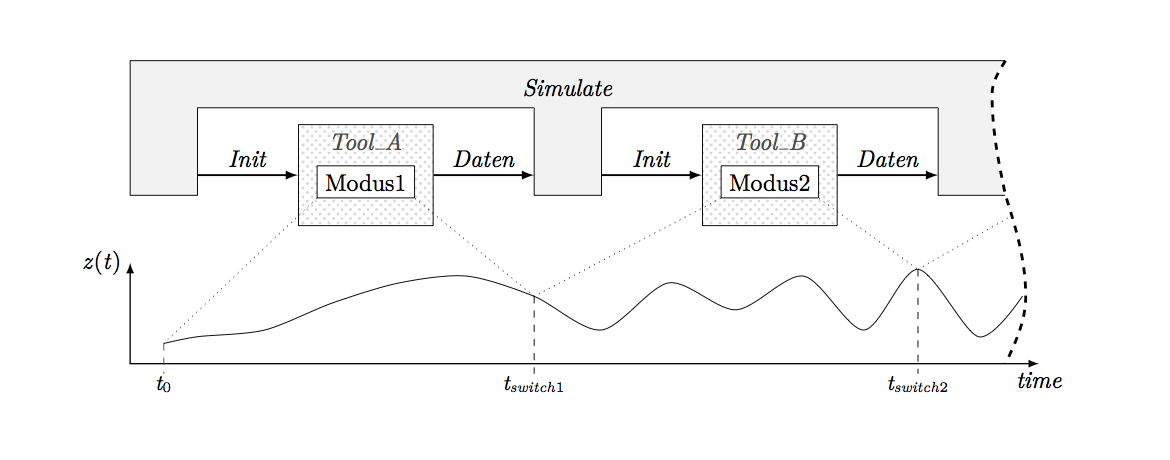
\includegraphics[width=1.0\textwidth,angle=0]{images/GettingStarted/simulation}
 \caption[General simulation procedure]{General simulation procedure}
 \label{fig:simulation}
\end{figure}

At the beginning the first mode must be identified and initialized. At every mode switch the simulation data of the just simulated mode will be read, saved and used to identify the next mode and to initialize that next mode. \\

The framework features an easily understandable object-oriented structure (see Figure \ref{fig:design}). There are three main classes which are important (and can be found in the \textit{src} directory).

 \begin{figure}[htb]
 \centering
 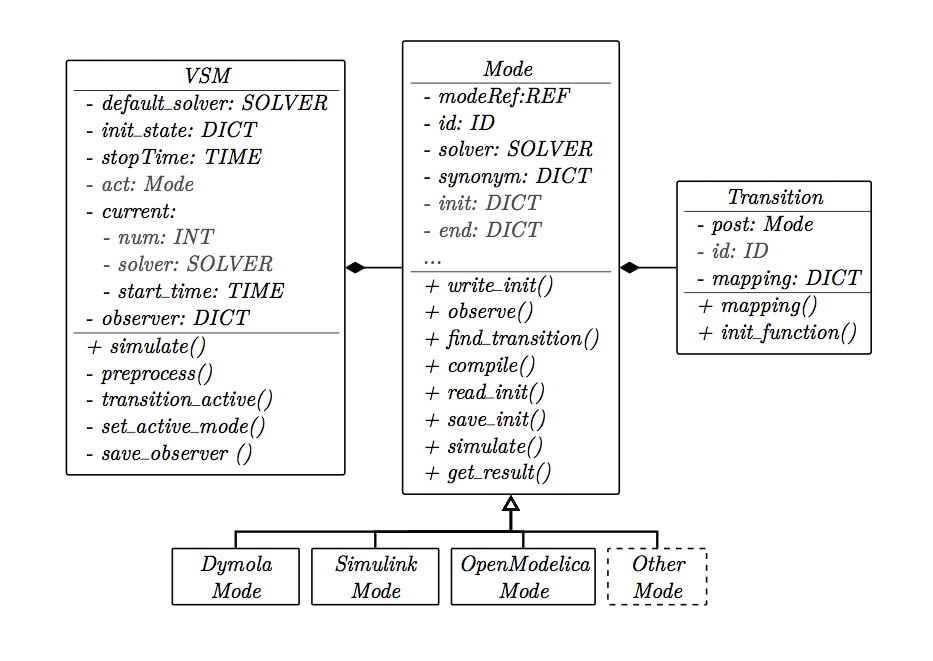
\includegraphics[width=1.0\textwidth,angle=0]{images/GettingStarted/FrameworkDesign}
 \caption[Object-Oriented Design of DySMo]{Object-Oriented Design of DySMo. This is not up-to-date and is not implemented in that way anymore but still shows the idea.}
 \label{fig:design}
\end{figure}

First you have the \textit{VSM} class (short for variable-structure model class). For every simulation of a variable-structure model exactly one instance of this class will be created. This instance provides some general attributes for the simulation (that can be set by the user) and the implementation of the basic functions which are needed to simulate the variable-structure model. In the \textit{VSM} class an \textit{observe} array containing the variables which should be observed and saved during the simulation, is provided and can be set.\\
Further the \textit{VSM} class provides attributes for the start and stop time of the simulation, for a default solver, for the initial state of the simulation (or the initial values of the first mode's variables) and attributes for the current simulating mode such as the simulation number, the used solver and the start time. \\
\\
The mode class represents the partial models that altogether form the variable-structure model.
Each mode corresponds with an independent (static-structure) model.
It is the task of the mode class to ensure communication, in particular simulation, with the underlying model.
It uses the Python Simulation Library to do so.
The modes are directly assigned to the \textit{VSM}.\\
Every mode provides a dictionary \textit{synonym} which maps the observed variables' names of the \textit{VSM} onto the corresponding mode's variables. Furthermore the modes have attributes for the solver, the init and the end state (or the initial and end values of the variables), a mode id and a \textit{modeRef} which references a mode uniquely. The simulation results of a mode's simulation are saved into a file, named due to the simulation number and the mode ID. The simulation number increases by one, everytime the current simulated mode switches. \\
\\
The transitions are assigned to the modes out of which they lead.
That means for a mode switch, that just the relevant subset of transitions has to be checked for the right one instead of the whole set. This is important for describing the model's structure.\\
The transition also provides a dictionary which maps the variables of the mode out of which it leads, onto the variables of the next mode. The initial state of the next mode can be modified by an \textit{init\_function} which can be specified in the transition, too.\\
\\
For creating a variable-structure model you need the mode's model files on the one hand and a \textit{Variable-structure description}-File on the other hand. The \textit{Variable-structure description}-File, called \textit{Config} from now on, defines the concrete structure of the variable-structure model. It describes loosely speaking the general properties, the number and properties of the modes, the needed transitions and the approach of visualizing the simulation results through plots. How this is done, is illustrated in the following section.

\subsection{Creating a variable-structure model}
 In this section a case study is designed to explain how you create and simulate a variable-structure model with DySMo. You can find the implemented model in \textit{sample/pendel}.
 
 \subsubsection{The cable pendulum}
 
Consider a cable pendulum which becomes a falling mass, once the centrifugal force is no longer sufficient to keep the pendulum on its circular path (see Figure \ref{fig:pendulum}).
 
 \begin{figure}[htb]
 \centering
 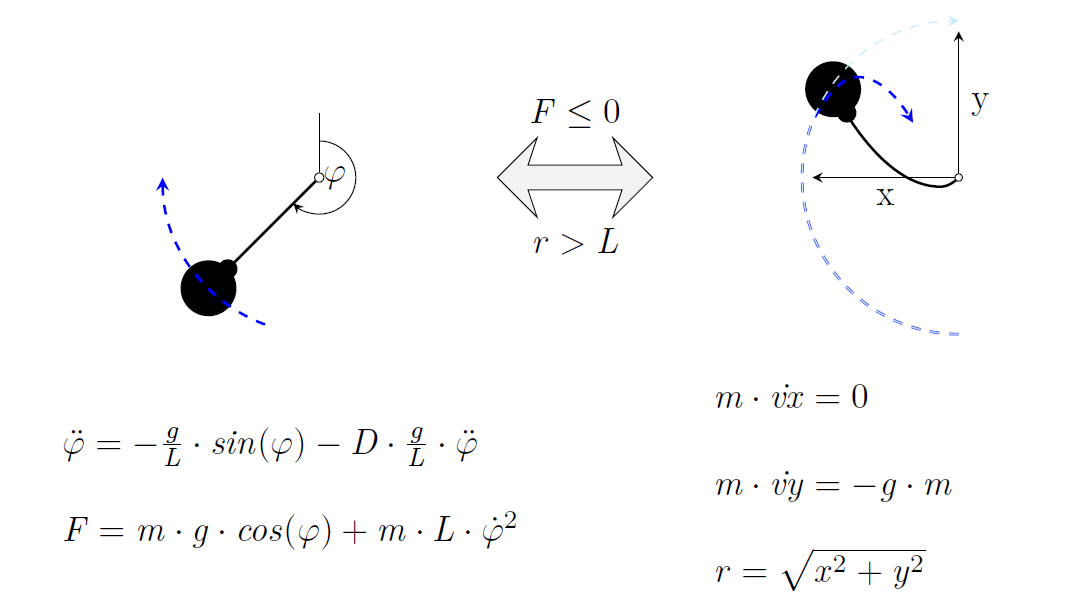
\includegraphics[width=0.7\textwidth,angle=0]{images/GettingStarted/pendulum}
 \caption[Physical representation of the cable pendulum]{Physical representation of the cable pendulum}
 \label{fig:pendulum}
\end{figure}

Once the mass falls into the cable again, the pendulum changes to its normal swing. As you can see in Figure \ref{fig:pendulum}, cartesian and polar coordinates are used in two different systems of equations to describe the normal swing and the falling mass. Thus, two modes are supposed to be implemented.

 \subsubsection{The Config-File}

For every variable-structure model you need to create a file that defines the variable-structure model.
In particular this file contains setting parameters for the variable-structure model itself, the single modes, the transitions and maybe some initial functions for initializing new modes.
The Config-File has to be written in Python and uses the classes that are already implemented in DySMo. The complete Config-File of the pendulum can be found in \textit{sample/pendel}. \\
\\
At first you should set the general model parameters (see Figure \ref{list:cfgmodelp}).

\lstset{language=python}
\begin{lstlisting}[frame=htrbl, caption={Pendulum Config.py - Model Parameters}, label={list:cfgmodelp}]
model.default_solver = Solver("dassl");
model.translate = True;
model.init = {};
model.startTime = 0;
model.stopTime = 10;
model.observe = ['x', 'y'];
\end{lstlisting}

Consider that the variable \textit{model} is always available in a Config-File, which is the single instance of the VSM class. There are different general model parameters for the variable-structure model you can set. You can choose the default solver (line 1), start and stop time of the simulation (line 4 and 5). If the parameter \textit{model.translate} is \textit{True}, your model and modes will be compiled before simulation (see line 2). If the models of the single modes have already been compiled, you can set this parameter to \textit{False} to save compilation time. It is recommended to leave this option \textit{True} to avoid mistakes.
In line 9 an array is created for the variables you want to observe (and maybe plot later). At this point you just list the names of the observed variables under which they will be saved after simulation.\\
\\
Next you should define the single modes of the variable-structure model (see Listing \ref{list:cfgmodesp}).

\lstset{language=python}
\begin{lstlisting}[frame=htrbl, caption={Pendulum Config.py - Modes}, label={list:cfgmodesp}]
#First mode
mode1 = Mode();
mode1.solver.tolerance = 1e-4;
mode1.modeRef = "pendulum.Pendulum_struc";
mode1.files = ["pendulum.mo"];
mode1.synonym = {'x' : 'x', 'y' : 'y'};

#Second mode
mode2 = Mode();
mode2.solver.tolerance = 1e-4;
mode2.modeRef = "pendulum.Ball_struc";
mode2.files = ["pendulum.mo"];
mode2.synonym = {'x' : 'x', 'y' : 'y'};
\end{lstlisting}

First a mode has to be declared (see line 2 or 9). After that you can set parameters of the mode like the solver tolerance (see line 3) or the solver that should be used. If you do not specify a solver, the default solver that is set in the general model parameters, is used. After that you have to state which model (see line 4 or 11) of which package file (see line 5 or 12) should be used for the mode.
Lines 5 and 12 specify which model files the mode consists of.
This is a list as models may need data from different files (for instance in Modelica).\\
Consider that these files must be located in the same directory as the Config-File. At last the variables of the model which should be observed, must be mapped to the variables you listed for the whole model (see line 6 and 13) in a \textit{dictionary}. You form tupels of the observed variables and the variables that represent them in the mode, in that order using colons.\\
\\
The next step is to declare the transitions from one mode to another. In this case you need a transition from the first mode to the second one and a transition the other way round (see Listing \ref{list:cfgtransp}). Consider that you cannot refer to any modes in the transitions that have not been declared yet.

\lstset{language=python}
\begin{lstlisting}[frame=htrbl, caption={Pendulum Config.py - Transitions}, label={list:cfgtransp}]
#Transition from mode 1 to mode 2
trans1_2 = Transition();
trans1_2.post = mode2;
trans1_2.mapping = 	{'x' : 'x', 'y' : 'y',  
				'vx': 'der(x)' ,  'vy':'der(y)'};

#Transition from mode 2 to mode 1
def speed(actMode, oldMode):
	actMode.set_initialValue('dphi', 0.0);

trans2_1 = Transition();
trans2_1.post = mode1;
trans2_1.mapping = {'x' : 'x', 'phi' : 'phi'};
trans2_1.init_function = speed;
\end{lstlisting}

First, you have to declare a transition (see line 2 or 11). Next you have to set the mode the transition leads to (see line 3 or 12). After that the variables which must be initialized, have to be specified. Therefore, you can specify a mapping dictionary or define an own function. If you use the mapping dictionary, tuples of variables must be formed (see line 4 or 13). The first variable is the one of the new mode that should be initialized. The second one is the variable of the old mode which should be used to initialize the new one. The variables are separated by colons and the tuples by commas again. Further you can initialize variables by defining an own function (see line 8-9). After defining an own function you can set the transition's init-function as that function (see line 14).\\
\\
Finally the transitions have to be added to the modes and the modes to the (variable-structure) model (see Listing \ref{list:cfgstm}).

\lstset{language=python}
\begin{lstlisting}[frame=htrbl, caption={Pendulum Config.py - Set Transitions and Modes}, label={list:cfgstm}]
#Set the transitions
mode1.transitions = [trans1_2];
mode2.transitions = [trans2_1];

#Set the modes
model.modes = [mode1, mode2];
\end{lstlisting}

For every mode the transitions which lead out of it, have to be set in an array (see line 2 and 3). Consider that the transition's ID refers to its position in this array, starting with one. That is important for designing the models of the modes. The same applies to the modes and the variable-structure model (see line 6).\\
\\
Now you have the possibility to create plots of the observed variables after simulation (see Listing \ref{list:cfgplot}).

\lstset{language=python}
\begin{lstlisting}[frame=htrbl, caption={Pendulum Config.py - Set Plots}, label={list:cfgplot}]
#Create plots
plot = VariablePlot();
plot.vars = {'y' : Color.MAGENTA};
plot.xAxisVar = 'x';
plot.drawGrid = 1; 
plot.labelXAxis = "x";
plot.labelYAxis = "y";
plot.fileName = 'pendulumplot.png';

#Set the plots
model.plots = [plot];
\end{lstlisting}

After simulation you get the plot of Figure \ref{fig:pendulumplot}.\\

 \begin{figure}[htb]
 \centering
 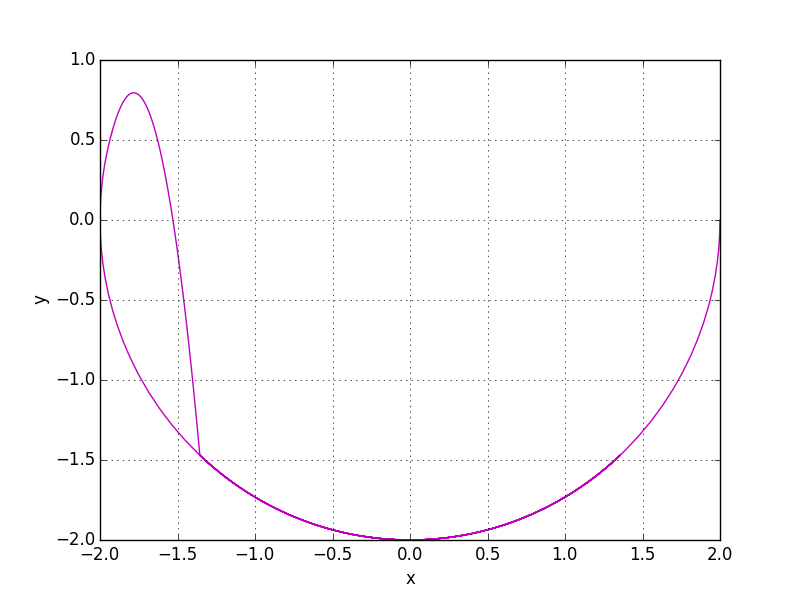
\includegraphics[width=0.7\textwidth,angle=0]{images/GettingStarted/pendulumplot}
 \caption[Pendulum - Plot]{Pendulum - Plot}
 \label{fig:pendulumplot}
\end{figure}

The plot shown in Listing \ref{list:cfgplot} is of type \textit{VariablePlot}. The framework provides two types of plots that can be used.
The \textit{VariablePlot} is a plot for creating a curve for (\textit{observed}) variables over all modes.
You can specify a color for the variable by indicating that in a dictionary as tuples of the variable name itself and the color of their curve (see line 3, Listing \ref{list:cfgplot}).
The second type is the \textit{ModePlot}.
For the \textit{ModePlot} the same attributes can be set as for the \textit{VariablePlot}.
The only difference is that the \textit{vars} attribute is not a dictionary anymore, but a simple array of variables.
The color of the curve will automatically change in accordance with the mode switches during simulation.

 \subsubsection{Transitions in the model file}

For a variable-structure model the modes need termination conditions which are specified in the corresponding models (see samples/pendel/pendulum.mo). For each mode the termination condition and the transition that leads to the next mode, has to be specified. Thus, every mode must have a variable named \textit{transitionId} (exactly in this spelling, code characters are case sensitive). Before the simulation of the active mode terminates, an integer value has to be assigned to this variable referring to the corresponding transition. As already mentioned the transition will be taken from the position in the mode's transition array according to this \textit{transitionID}.\\
\\
For the cable pendulum example every mode has just one transition which leads out of it. Thus the \textit{transitionId} is set to 1 before terminating. In Listing \ref{list:pmodel} the mode of the normal swing is shown (the second mode). It is implemented in Modelica.
\lstset{language=modelica}
\begin{lstlisting}[frame=htrbl, caption={Pendulum Model File - pendulum.mo}, label={list:pmodel}]
model Pendulum_struc
  extends Pendulum_phi;
  Integer transitionId(start = 0);
equation 
    when F <= 0 or terminal() then
    transitionId = 1;
    terminate("Pendulum to ball");
    end when;
end Pendulum_struc;
\end{lstlisting}

 The \textit{transitionId} is set to 0 by default (see line 3). Once the termination condition is met (see line 5), the \textit{transitionId} is set to 1 before terminating this mode. According to Listing \ref{list:cfgstm} the first transition will be chosen out of the array in line 3 which is \textit{trans2\_1}.

\subsection{Simulation}

To simulate a model you have to call:
\lstset{language=bash}
\begin{lstlisting}
python PathToDySMo/DySMo.py PathToYourModel/ModelConfig.py
\end{lstlisting}

For Windows users we also included a simple Batch-file to run a model through Drag-and-Drop.
However, this method might fail because of missing administrator rights.
To use the Batch-file, simply drag the Config.py file an drop it on the run.bat file (see Figure \ref{fig:startingsimulation}).

 \begin{figure}[htb]
 \centering
 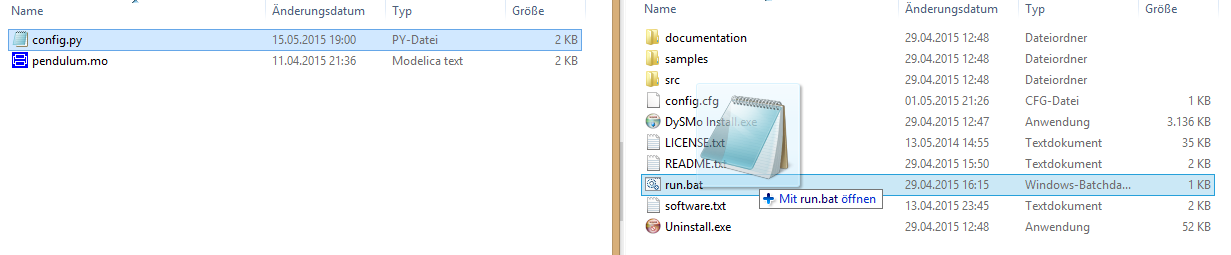
\includegraphics[width=1.0\textwidth,angle=0]{images/GettingStarted/DragDrop}
 \caption[Starting the simulation]{Starting the simulation}
 \label{fig:startingsimulation}
\end{figure}

The simulation will start and simulate the single modes according to the transitions, always starting with the first mode (you have set in line 6, Listing \ref{list:cfgstm}).
After simulation the Python console should look like Figure \ref{fig:pconsole}.\\

 \begin{figure}[htb]
 \centering
 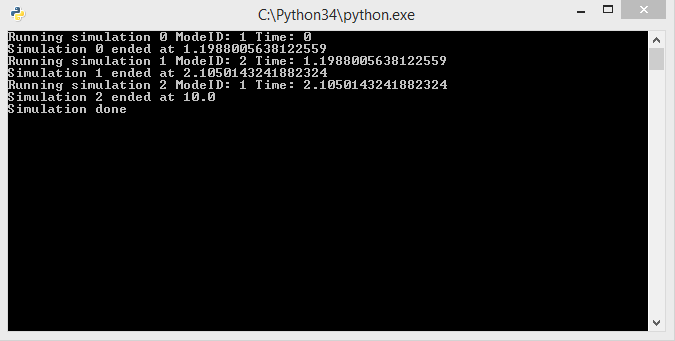
\includegraphics[width=1.0\textwidth,angle=0]{images/GettingStarted/pythonconsole}
 \caption[The python console after simulation]{The python console after simulation}
 \label{fig:pconsole}
\end{figure}

Now lets take a closer look on the folder that contains your model (in this case  \textit{sample/pendel}). Now it contains some more files and an additional folder named \textit{result} (see Figure \ref{fig:modelfolder}).

 \begin{figure}[htb]
 \centering
 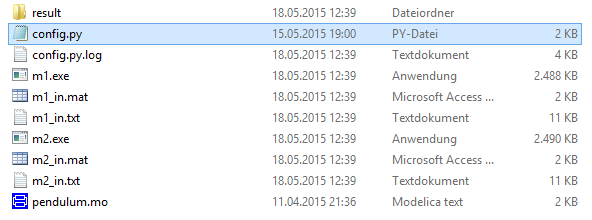
\includegraphics[width=1.0\textwidth,angle=0]{images/GettingStarted/modelfolder}
 \caption[Folder of the variable-structure model after simulation]{Folder of the variable-structure model after simulation}
 \label{fig:modelfolder}
\end{figure}

In the \textit{config.py.log} file you can find general information about the simulation such as the overall simulation time, the simulation and compilation time of each mode. The exe-files \textit{m1.exe} and \textit{m2.exe} are compiled versions of the modes. The files \textit{m1\_in.txt} and \textit{m2\_in.txt} contain further information for the modes' initializations such as initial values of the variables, solver informations and so on. The files  \textit{m1\_in.mat} and \textit{m2\_in.mat} contain the initial values of the variables that are loaded into the simulation tool before simulating the according mode. The simulation results are saved in the folder \textit{result} (see Figure \ref{fig:result}).

 \begin{figure}[htb]
 \centering
 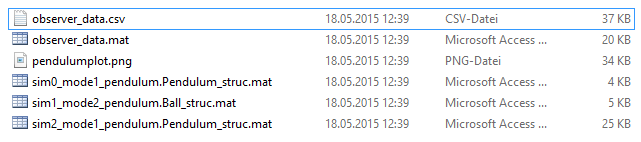
\includegraphics[width=1.0\textwidth,angle=0]{images/GettingStarted/resultfolder}
 \caption[Simulation results]{Simulation results}
 \label{fig:result}
\end{figure}

In this folder you can find a mat-File containing the observer variables' values over the complete simulation and you can find mat-files referring to the single modes. Finally also the plots which are set in the Config.py file, can be found here.
